% Research Paper for MICS 2014
% by David Donatucci, Kirbie Dramdahl, and Nic McPhee

\documentclass[12pt]{article}

\setlength{\oddsidemargin}{0in}
\setlength{\evensidemargin}{0in}
\setlength{\topmargin}{0in}
\setlength{\headheight}{0in}
\setlength{\headsep}{0in}
\setlength{\textwidth}{6in}
\setlength{\textheight}{9in}
\setlength{\parindent}{0in} 

\usepackage{parskip}
\usepackage{times} %For typeface
\usepackage{graphicx}
\usepackage{algorithm}
\usepackage{algorithm,algorithmic}
\usepackage[justification=centering]{caption}[2007/12/23]
\usepackage{url}
\sloppy

\newcommand{\inset}[1]{$\in \{ {#1} \}$}

\newcommand{\citep}[1]{\cite{#1}}
\newcommand{\PPLR}[1]{$\eta_M$}
\newcommand{\LLR}[1]{$\eta_L$}

\DeclareGraphicsRule{.tif}{png}{.png}{`convert #1 `dirname #1`/`basename #1 .tif`.png}

\title{Analysis of Genetic Programming Ancestry Using a Graph Database}

\author{
 		David Donatucci, M. Kirbie Dramdahl, and Nicholas Freitag McPhee\\
        Division of Science and Mathematics\\
        University of Minnesota, Morris\\
        Morris, MN 562367\\
        donat056@morris.umn.edu\\
        dramd002@morris.umn.edu\\
        mcphee@morris.umn.edu\\
}
\date{} 

\begin{document}
\pagestyle{plain}

\maketitle

\begin{abstract}

Genetic programming is an artificial intelligence approach that uses basic properties of biology such as fitness, mutation, and crossover to manipulate a population of functions. These functions are typically represented as trees. By performing mutations and crossovers over many generations, genetic programming attempts to evolve these trees toward a desirable result. The strength of a tree is determined by its fitness, which is calculated based on the evaluation of the tree at a series of points compared with the target function at the respective points. The evolution process is achieved in a similar manner to natural selection, where trees with stronger fitness have a better chance of reproduction, and weaker trees tend to be removed from the population.

In this project, our objective is to map the ancestry of these trees and how they change over time using a graph database. Graph databases are relatively new, and provide features such as relational queries to obtain data that would be difficult with standard databases. In traditional databases, as data sets increase in size, recursive queries become extremely inefficient. By comparison, with a graph database such as Neo4j, recursive queries with large data sets remain relatively constant. Since genetic programming involves a significant number of trees and a multitude of generations, graph databases allow for efficient querying of ancestry that would not be possible with more traditional database systems such as SQL.  

Our hope is that by recording and analyzing tree ancestry, we will be able to obtain more substantial data regarding the natural selection process undertaken in genetic programming. Perhaps most significantly, we hope to discover where trees show significant improvement in fitness and how those improvements are obtained. This will allow for a better understanding of how genetic programming works and provide details for future improvements in the evolutionary computation field.

\end{abstract}

\section{Introduction} \label{sec:intro}

Genetic programming (GP) is an artificial intelligence approach that implements the basic principles of biology to discover solutions to a user defined problem. Like biological evolution, genetic programming consists of organisms called individuals which are evaluated based upon their fitness. Individuals most suited to their environment will have a stronger fitness and individuals with stronger fitness typically produce more offspring than those with weaker fitness. Over many generations, descendants generally have stronger fitness than their ancestors from previous generations.

Genetic programming systems are great tools for discovering solutions to complex problems involving many variables that would be extremely difficult to solve by other means. Genetic programming has applications in chemistry, electronic circuit design, economics, and many other applications. 

While genetic algorithms have clearly been successful in a variety of settings, it is often challenging to determine why this is true. In order to reach a greater understanding of the processes involved in genetic programming, it is necessary to examine the internal interactions of individuals within a run, rather than simply statistical summaries of the final results. Even simple GP runs can generate very large data sets, however, especially if one records all the individuals and relationships from every generation.

Databases are a natural tool for handling such large data sets, but important questions and queries for evolutionary computation (EC) work are difficult when using relational databases. A natural question when analyzing an EC run, for example, would be to find all the ancestors of the ``winning'' individual. If we used a relational database, we might store the IDs of the parents along with each individual. A single query would then return the parents of an individual, but then additional queries (one per parent) would be needed to get the set of grandparents, and additional queries (one per grandparent) would be needed to get the set of great grandparents, etc. Assuming two parents per individual, the number of queries will then grow as $O(2^n)$ where $n$ is the number of generations back we want to collect ancestors for, making this approach totally unfeasible for a host of interesting and important questions.

New graph database technologies, however, have the potential to allow us to easily perform these sorts of queries and analyze important dynamic properties of GP runs. In graph databases one stores nodes and relationships, such as individuals and their relationships to their parents, and the query language makes it easy to search for paths through the graph having specified properties. This makes it fairly trivial to ask important ancestry questions about a run; the query \texttt{MATCH (n)<-[*]-(p)}, for example, will find all the ancestors $p$ of some individual $n$. (The details of graph databases and the Cypher query language will be described in more detail in Section~\ref{sec:Graph Databases}.)

This paper demonstrates the usefulness of graph databases in recording and analyzing data produced by genetic programming systems. A description of genetic programming is provided in Section \ref{Genetic Programming}, and Section \ref{sec:Graph Databases} discusses graph databases. Section \ref{sec:experiments} provides details on how we set up a run of our experiment. In summary, the results of our work are presented in Section \ref{sec:results}, and ideas for future implementation and applications of this work, are presented in Section \ref{sec:conclusion}.

\section{Genetic Programming} \label{Genetic Programming}

Genetic programming is based around the interactions of individuals. Individuals are equivalent to organisms in the biological sphere. As in the biological sphere, a group of individuals makes up a population. In the process of biological evolution and natural selection, organisms within a population compete in order to survive and reproduce. Those individuals best adapted to their environment have the best chance of fulfilling these objectives.  In genetic programming, individuals compete for the same reasons, but here it is those individuals that provide a best fit or solution to the user-defined problem that have the best odds. The goal of genetic programming, is to produce an individual that provides the optimal solution.

The effectiveness of the solution an individual provides is determined by the fitness of the individual. The fitness is the difference between the target function and the function of the individual. The lower the fitness, the better the solution fits the initial problem. An individual with a solution that perfectly fits the problem would have a fitness of zero. Therefore, at the conclusion of a genetic programming run, it is desirable to have produced one or more individuals with fitness of or approaching zero.

At the start of a run, the population is filled with randomly generated individuals. The individuals within this population then compete in order to pass their code on to the next generation, similar to biological evolution. This competition, in genetic programming, is called the tournament, where a specified number of individuals are randomly chosen from the population, and those with the best fitness are selected to produce the next generation. These selected individuals can propagate their genetic material onto the next generation by one of three transformation types. The first and most common method is crossover, comparable to sexual reproduction, where two individuals are selected from the current generation, and elements from each selected individual are combined to form a new individual in the next generation. The second method is mutation, in which an individual is selected and randomly altered, much like biological mutation. The third and final method is reproduction, where an individual is copied to the next generation, akin to asexual reproduction. There is also an alternative form of reproduction known as elitism. Elitism occurs when particularly fit individuals are copied to the next generation by merit of their fitness alone. Crossover, mutation, and reproduction are utilized many times, across multiple generations, until an ideal or approximate solution is found~\cite{poli08:fieldguide}.

\section{Graph Databases}
\label{sec:Graph Databases}

The graph database Neo4j was used collect data generated by runs of the genetic programming algorithm. This section further describes Neo4j, its query language Cypher, and the various advantages they hold over relational databases in recording and accessing information that relies heavily on recursion.

Neo4j is a form of data management system based upon a graph. Information is stored by means of vertices and edges, commonly referred to as nodes and relationships, respectively~\cite{GraphDatabases:2013}. In our work, nodes represent individuals, and relationships represent the transformation types between individuals.

Cypher allows data to be readily extracted from Neo4j. There are three fundamental elements to queries in Cypher. The START clause specifies a starting location in the database, selecting the node or relationship where the query will begin. The RETURN clause specifies which nodes, relationships, or properties should be returned to the user. The MATCH clause is the main section of a query. MATCH specifies what the query will discover. To write the MATCH clause nodes and relationships are drawn with ASCII characters. A node is indicated by parenthesis ( ), and relationships are composed of dashes along with greater-than or less-than signs to indicate the direction of the relationship. Inside of brackets [ ] between the dashes are the specified relationship names prefixed by a colon~\cite{GraphDatabases:2013}. In the example query, ‘example1’ we see that the START clause indicates the node to begin the query, the MATCH clause finds all nodes that are children of the starting node, and the RETURN clause yields the starting node and all nodes that are children of that node.

\begin{verbatim}
START parent=node(43)
MATCH (parent)-[:PARENTOF]->(child)
RETURN parent, child;
\end{verbatim}

This query produces the results in Figure \ref{fig:exampleQuery}.
\begin{figure}[tb]
 \centering
 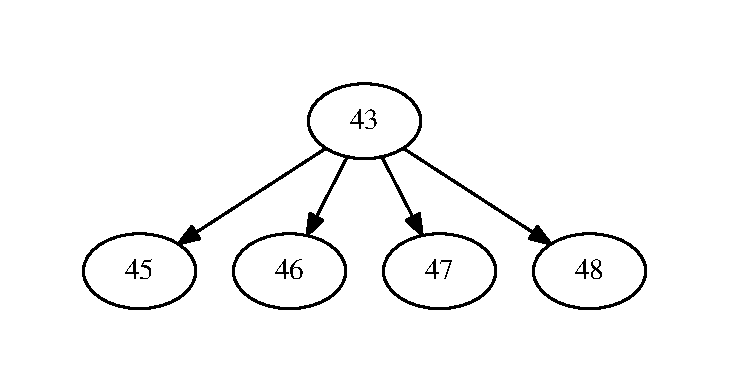
\includegraphics[height=0.30 \textwidth]{parents}
 \caption{Results of Example Query}
 \label{fig:exampleQuery}
\end{figure}

The advantage of a graph database over relational databases relevant to our research was performance. As the dataset grows, relational databases tend to become highly inefficient, as the entire dataset must be searched in response to each query. In graph databases, however, the portion of the dataset that must be searched is limited because the query will only search along an available path connected by relationships. Therefore, this structure allows queries to remain efficient~\cite{GraphDatabases:2013}.

\section{Experimental Setup} 
\label{sec:experiments}

This section explains the details of the configurations used for this research. Subsection \ref{sec:GPSetup} covers setup of the genetic programming algorithm, and Subsection \ref{sec:Neo4jSetup} discusses setup of the graph database Neo4j.

\subsection{Genetic Programming Setup}
\label{sec:GPSetup}

In all of the runs, the configurations remained consistent, with the exception of population size. In the several runs that were performed, the population size was either 1,000, or 10,000. The target function was as follows:
\[
    \sin(x)
\]
where the value of the variable $x$ ranged from 0 to 6.2, increasing by steps of 0.1. The constants allowed were doubles that ranged between -5 and 5, and $x$ was the sole variable. The operations allowed in order to achieve an optimal solution to the target were the binary operations: addition, subtraction, multiplication, and division. Since division is undefined when the denominator is equal to zero, we implemented protected division. In our protected division, if the denominator equals zero, then regardless of the numerator value the output will be one. The reason we chose the output one for protected division is so there would not be a discontinuity in the function $x/x$ when $x = 0$. Therefore, when evolving $x/x$ in a individual we will continue to obtain the value one.

In our system, individuals contain two items: a function called the tree, and the tree's fitness. trees are represented in prefix notation by arrays containing variables, constants, and operators. Prefix notation is a way to write  a function that places the operator before its arguments. For example, a tree of the function $x + (x * 4)$ would be represented by the following array: [+,~x,~*,~x,~4]. The tree's fitness is the sum of the absolute error between the target function and the tree at all predetermined variable values. The absolute error is  the measured value of a quantity $x_{0}$ and its actual value $x$, given by the equation $\Delta x=x_{0}-x$.

After the tree's fitness is computed, we add a constant to the fitness as a means to penalize particularly large trees. This encourages trees to not become excessively large, and is commonly referred to in genetic programming as bloat control. We selected this constant to be a hundredth of the tree size. This implementation of bloat control is relatively weak in the beginning of a run where trees usually have larger fitnesses (therefore not penalizing them unreasonably), but has a significant impact later in the run, where trees should have smaller fitnesses.

To create the initial population, we implemented an algorithm called PTC2~\cite{Luke2013Metaheuristics}. The PTC2 algorithm creates trees by randomly adding operators to an array (leaving blank indices where appropriate for arguments) until a specified length is reached. The blank indices are then filled by leaves (variables and constants). Leaves consist of 63\% variables and 37\% constants.

In order to selection those individuals which will produce the next generation, we  implemented tournament selection. In our tournament, two individuals are selected from the entire generation. The individual with the best fitness of the two selected is chosen to propagate its code in some capacity on to the next generation. This process repeats for the creation of every individual in the next generation.

As discussed previously, individuals may pass on their code by three different means: crossover, mutation, and reproduction. Crossover makes up 90\% of all transformations, mutation 1\%, and reproduction accounts for the remainder. Reproduction is relatively straightforward. The individual which wins the tournament is simply copied on to the next generation. A variation on reproduction is elitism, where an individual is copied to the next generation by merit of it fitness. In other words, within a generation, 1\% of individuals with the best fitness skip tournament and are simply copied over to the next generation. Mutation and crossover are more complex processes, and will be covered in the following paragraphs.

Mutation begins in a similar manner to reproduction. Two individuals are selected from the population to enter the tournament, and the winner is chosen for mutation. However, rather than simply copying this individual on to the next generation, a random index from within the tree is selected. If the index is a operator, the subtree starting at that operator is removed. A subtree is a section of a tree that is itself a valid tree. Otherwise, if the index is a leaf, the index is removed. In both cases, the removed index or indices are replaced by a new subtree generated by PTC2 that is at most half the size of the original tree. This limitation has been put in place to help in controlling bloat.

Crossover differs from the previous transformations in that it makes two calls to the tournament in order to receive two individuals to produce a single child individual in the next generation. The first tournament results in a root parent. Within this parent, similar to mutation, a random index is chosen. If the index is an operator, the subtree is removed, otherwise only the index is removed. The removed index or indices are then replaced by a subtree randomly selected from the individual that won the second tournament.

\subsection{Neo4j Setup}
\label{sec:Neo4jSetup}

In Neo4j, we set nodes to be individuals and defined their ancestry as relationships. Inside each node, we inserted several attributes belonging to an individual. In addition to the tree and fitness, all nodes also include the penalized fitness, the generation number, the transformation type, the run id (used to differentiate between different runs), and a unique id (used for identifying the specific node). For individuals produced by either crossover or mutation, the ``cut point'' (the index at which the root parent was altered by a transformation) is also included as an attribute. These attributes are summarized in Table~\ref{tab:individualAttributes}.
\begin{table}[tb]
\begin{center}
\resizebox{15cm}{!}{
\begin{tabular}{|l|r|r|r|r|r|r|r|r|}
    \hline
    \multicolumn{9}{|c|}{\textbf{Individual Attributes}} \\
    \hline
    \textbf{Transformation} & \textbf{Tree} & \textbf{Fitness} & \textbf{Penalized Fitness} & \textbf{Generation Number} & \textbf{Transformation Type} & \textbf{Run ID} & \textbf{Unique ID} & \textbf{Cut Point} \\ \hline
    Elitism & X & X & X & X & X & X & X & \\
    Reproduction & X & X & X & X & X & X & X & \\
    Mutation & X & X & X & X & X & X & X & X \\
    Crossover & X & X & X & X & X & X & X & X \\
    \hline
\end{tabular}
}
\caption{Chart summarizing attributes that are recorded for individuals produced by each transformation type.}
\label{tab:individualAttributes}
\end{center}
\end{table}

Each individual has a relation to its parent (or parents in the case of crossover). To distinguish between each type of transformation, different types of relationships are used. These relationships are demonstrated in Table~\ref{tab:relationshipTypes}.
\begin{table}[tb]
\begin{center}
\begin{tabular}{|l|l|}
    \hline
    \multicolumn{2}{|c|}{\textbf{Relationship Types}} \\
    \hline
    Reproduction & PARENTOF \\
    Elitism & ELITISM \\
    Mutation & MUTANTOF \\
    Crossover Root & ROOT\textunderscore XOOF \\
    Crossover Non-Root & NONROOT\textunderscore XOOF \\
    \hline
\end{tabular}
\caption{On the left are the various transformation types and on the right are the relationship types assigned to each in the Neo4j database. Notice that crossovers have two relations because two parents were selected in tournament.}
\label{tab:relationshipTypes}
\end{center}
\end{table}

\section{Results} \label{sec:results}

To obtain the results presented here, we completed six runs at population 1000, and one 10000 run. From these runs, we were able to retrieve a variety of interesting data within a reasonable amount of time. The following are the questions we asked of the database:
\begin{itemize}
\item \textit{How many individuals in the initial generation have any root parent descendants in the final generation?}
\item \textit{How well do mutations perform against crossovers where the root parent is more fit than the non-root parent, and vice versa?}
\item \textit{Do a group of individuals have a common ancestor and in what generation does that ancestor occur?}
\item \textit{What does the fitness of the ``winning'' line look like over time?}

\end{itemize}

To answer the first question, we implemented the following query:

\begin{verbatim}
MATCH (startNode:Individual {generation: 1})-
[:ELITISM|PARENTOF|MUTANTOF|ROOT_XOOF*99]->
(endNode:Individual {generation:100})
RETURN distinct id(startNode), startNode.penalizedFitness;
\end{verbatim}

The MATCH statement describes that s and n are individuals in generation one and one hundred respectively using indexing. The relationship between them must be elitism, reproduction, mutation, or root parent crossover and must have a path depth of 99. The RETURN statement returns all individual ids along with its fitness in the initial generation that fit the criteria. This query produces the set of individuals that have descendant in the final generation. These individuals and their penalized fitness are represented in Table \ref{tab:descendantsTable}.
\begin{table}[tb]
\begin{center}
\begin{tabular}{|r|r|}
    \hline
    %\multicolumn{2}{|c|}{\textbf{First Generation Individuals with Final Generation Descendants}} \\
    %\hline
    \textbf{Individual} & \textbf{Penalized Fitness} \\ \hline
    2595 & 38.9820979981526 \\
    3325 & 40.36373034994929 \\
    \hline
\end{tabular}
\caption{List of individuals in the initial generation of the 10K run which produced root descendants in the final generation.}
\label{tab:descendantsTable}
\end{center}
\end{table}

This data demonstrates that, at least in this specific instance, all 10,000 individuals in the final generation can be traced back along their root parent line to only two individuals in the initial generation. This, in support of data gathered by McPhee and Hopper \cite{mcphee1999analysis}, indicates that the percentage of initial individuals with direct descendants in the final generation is relatively small. Furthermore, while neither of these individuals demonstrated the best initial fitness (24.18), both do appear in the top 5\% of fit first generation individuals. Whether this high fitness rate is consistent across multiple runs is unclear.

To determine the effectiveness of mutation versus crossover we wrote several queries similar to the following:

\begin{verbatim}
//Count total number of crossovers

MATCH (r)-[:ROOT_XOOF]->(c)<-[:NONROOT_XOOF]-(n)
RETURN count(distinct c);

//Count total number of crossovers fitting the description

MATCH (r)-[:ROOT_XOOF]->(c)<-[:NONROOT_XOOF]-(n)
where c.penalizedFitness < r.penalizedFitness 
     AND r.penalizedFitness < n.penalizedFitness
RETURN count(distinct c);

\end{verbatim}

These two queries above specifically identified the total number of crossovers and the number of root crossovers where the child was more fit than either parent and the root parent was more fit than the non-root parent. The other two cases, mutation and non-root crossover (the child was more fit than either parent and non-root parent was more fit than the root parent), represented in Figure \ref{fig:improvedFitness} had similar structures. The results of this query may be seen in Figure \ref{fig:improvedFitness}.

\begin{figure}[tb]
 \centering
 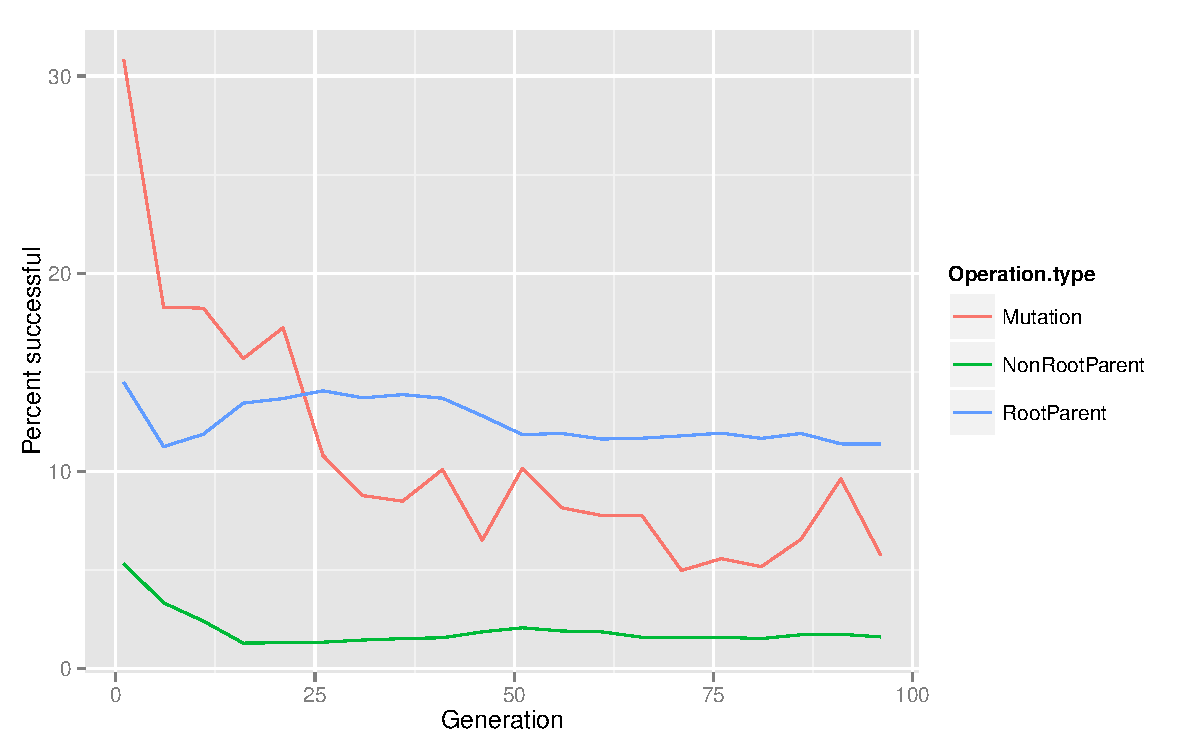
\includegraphics[height=0.68\textwidth]{Blocked_success_percentages}
 \caption{Percentage of Cases Where the Child is Fitter Than the Parent Over Five Generation Blocks in 10K Run}
 \label{fig:improvedFitness}
\end{figure}

To confirm the data we found in Figure~\ref{fig:improvedFitness}, we used the same queries on three 1K runs to obtain the graph in Figure~\ref{improvedFitness1K}. Again, we obtained similar data. In the first generations, mutation produced children that were better than their parents over 30\% of the time. As time progressed, the success of mutation decreased dramatically as time progressed dropping as low as ??5??\% of the time. On the other hand, the crossover percentages stayed relatively constant with the exception of the first ten generations of non-root crossover. Notice that the crossover variances were very small, meaning that crossover is a stable transformation over time. 

\begin{figure}[tb]
 \centering
 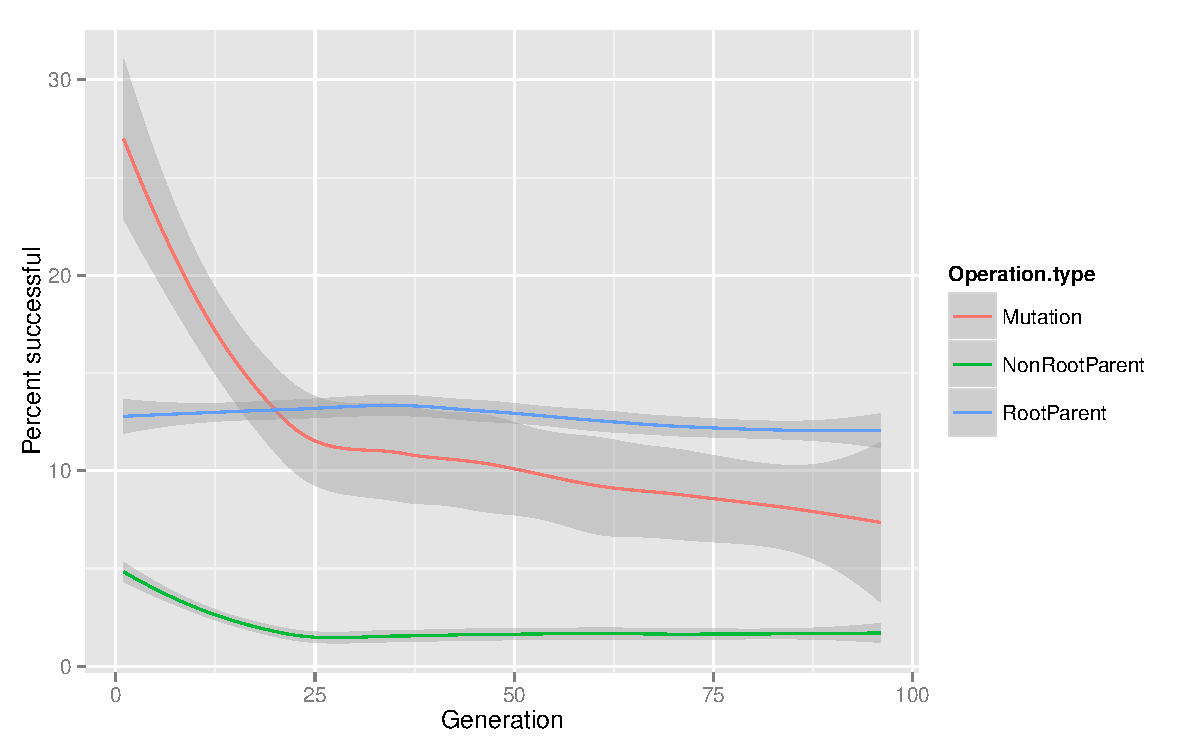
\includegraphics[height=0.68\textwidth]{Percent_successful_Axiom_1K_runs}
 \caption{Percentage of Cases Where the Child is Fitter Than the Parent Over Five Generation Blocks in Three 1K Runs. Shadows indicate the variance between each of the three runs.  }
 \label{fig:improvedFitness1K}
\end{figure}


To find a common ancestor of entire last generation, we executed the following query:   

\begin{verbatim}
MATCH (child:Individual {generation: 100})
<-[:ELITISM|PARENTOF|MUTANTOF|ROOT_XOOF*0..]-(parent)
<-[rel:ELITISM|PARENTOF|MUTANTOF|ROOT_XOOF]-(grandparent)
RETURN distinct id(parent), type(rel), id(grandparent);
\end{verbatim}

\begin{figure}[tb]
 \centering
 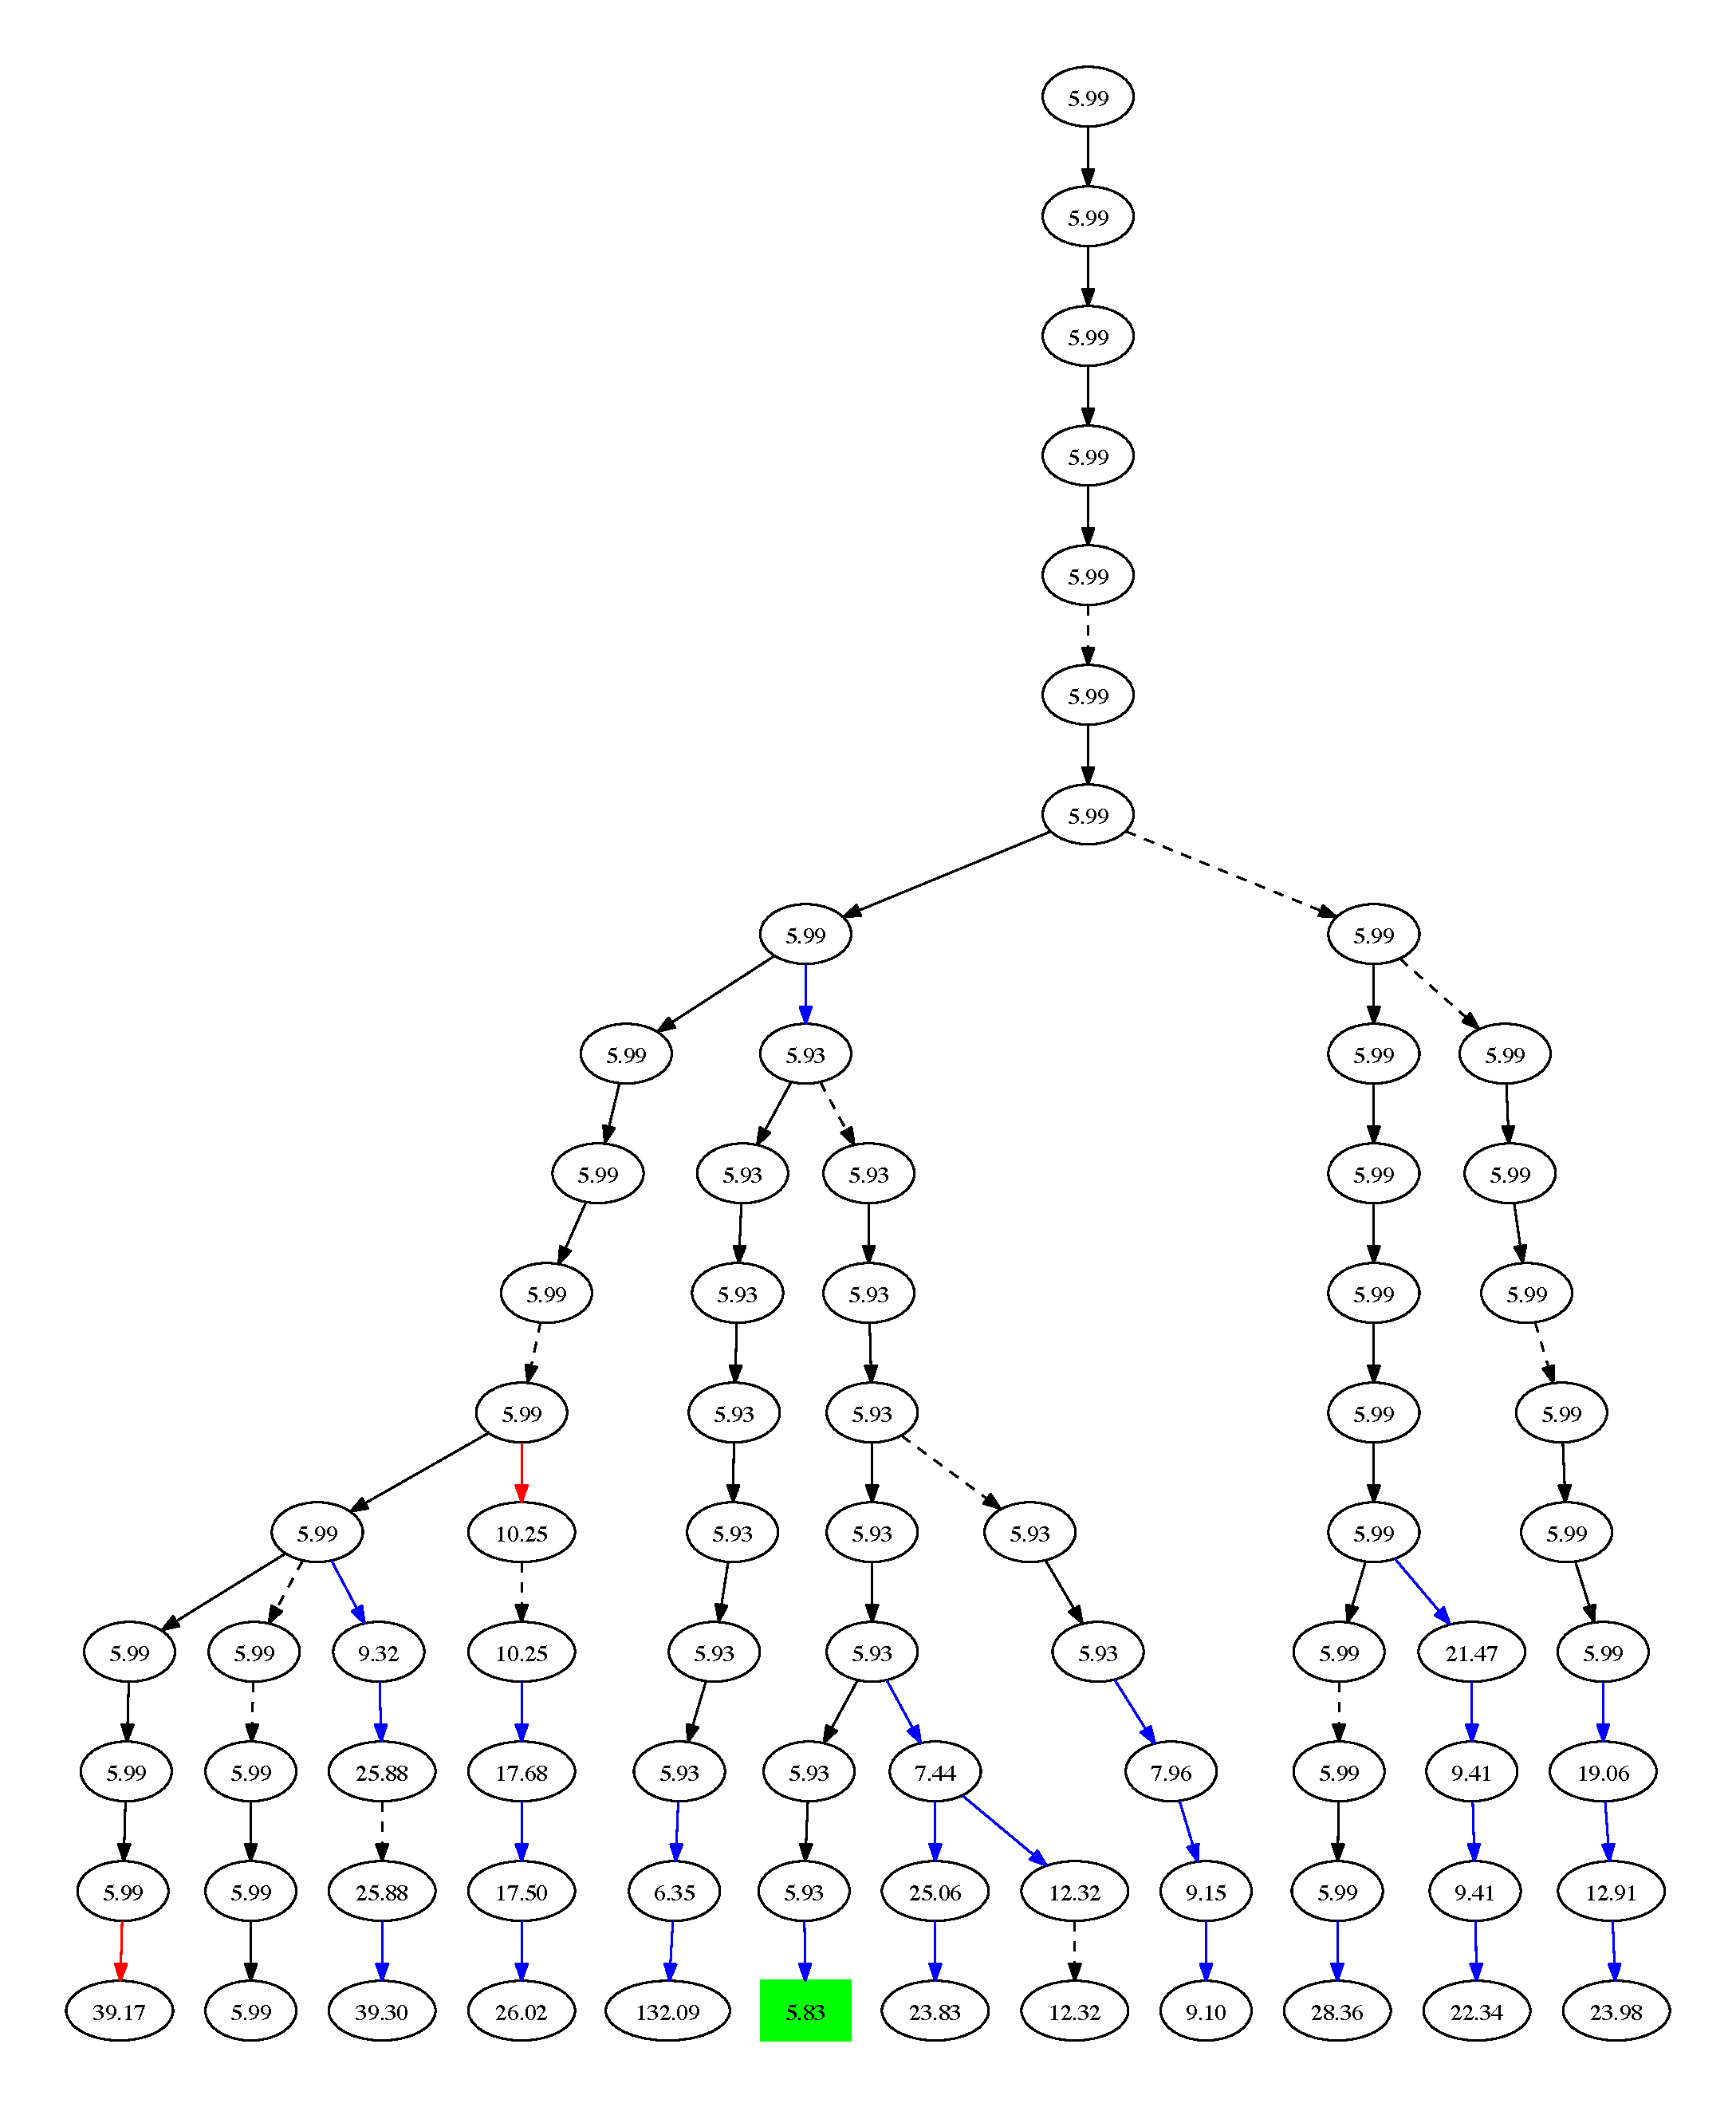
\includegraphics[width= \textwidth]{subset_confluence_trimmed}
 \caption{Results of finding the common ancestor between 11 random individuals and the ``winner'' highlight by a green box. Mutations relationships are highlighted by red arrows. Crossovers are blue arrows. Reproduction is a dotted black line and elitism is a solid black line.}
 \label{fig:exampleQuery1}
\end{figure}

From this query we found several interesting occurrences. In finding a common ancestor, we can assume that this ancestor carries certain positive traits. This information may be relevant in determining if traits other than fitness give an individual  chance of survival. In the 10K run, two distinct species were produced. One species flourished, accounting for 99.76\% of the final population while the second species consisted of only 24 individuals. These two species are descended from the individuals presented in Table~\ref{tab:descendantsTable}. While there are two individuals that are direct ancestors, descendants of the more fit individual predominated. Given more time, the second species most likely would have gone extinct.

The fourth and final question asked was answered by the following query:
\begin{verbatim}
start n=node(99000) 
match ps = (n)<-[r:ELITISM|PARENTOF|ROOT_XOOF|MUTANTOF*]-(p) 
return distinct ps;
\end{verbatim}

From this query, we obtained a graph of the entire root line of the ``winning'' individual. From this graph, we were able to abstract the fitness of each individual in the line. This same process was repeated for the non-root line. The resulting information regarding the fitness of both root and non-root ancestors of the most fit final individual over all generations is presented in Figure \ref{fig:rootVsNonrootFitness}. 
\begin{figure}[tb]
 \centering
 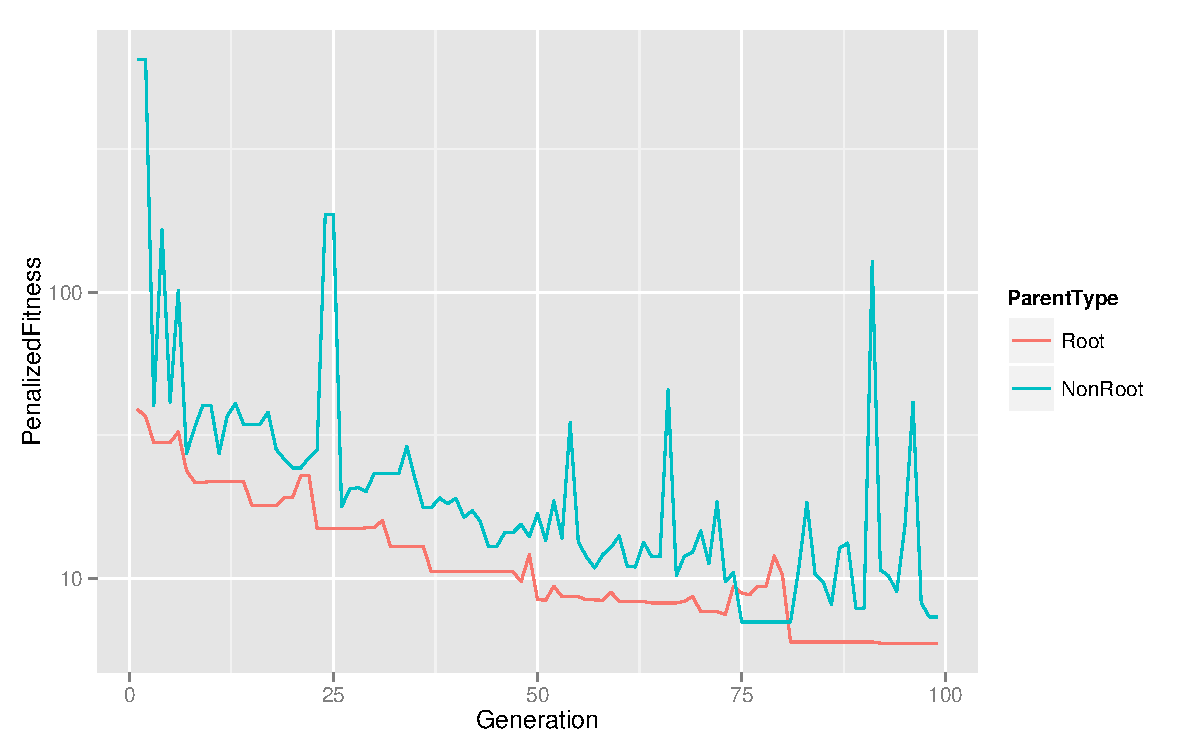
\includegraphics[height=0.68\textwidth]{Root_vs_nonroot_line_fitnesses}
 \caption{Root Versus Non-Root Fitness in Ancestry of Best Tree from Final Generation of a 10K Run}
 \label{fig:rootVsNonrootFitness}
\end{figure}

As can be seen in Figure \ref{fig:rootVsNonrootFitness}, while root parent fitness steadily decreases over time, no such pattern exists for non-root fitness. This implies that the root lineage is far more important in determining the overall success of a specific individual than the non-root lineage.

\section{Conclusions} \label{sec:conclusion}

A critical point is that graph databases like Neo4j don't make anything possible that was once impossible; they instead make these things vastly simpler and allow open-ended exploration. Each of the queries and questions we've discussed could be handled by, for example, special purpose code added to the evolutionary system to specifically capture that specific information. Many, if not most, of these have no doubt been addressed in a piecemeal fashion by previous research. Researchers observed~\cite{mcphee1999analysis} nearly 15 years ago, that root parent lineages were significant, and that these lineages quickly coalesced into a shared common ancestor, but that was using a specialized custom system to track that data, and there has been limited follow-up by others since then. We suspect a significant reason for the lack of similar work is simply the effort required to collect and analyze the substantial amount of data this entails, and the lack of good tools to simplify that process.

\section*{Acknowledgements}

\bibliographystyle{acm}
\bibliography{MICS_2014}

\end{document}
